\documentclass[12pt, a4paper, oneside]{ctexart}
\usepackage{amsmath, amsthm, amssymb, bm, color, framed, graphicx, hyperref, mathrsfs,enumerate,colortbl}
\title{\textbf{第四次作业}}
\author{1907402030 熊雄}
\date{\today}
\linespread{1.15}
\definecolor{shadecolor}{RGB}{241, 241, 255}
\newcounter{problemname}
\newenvironment{problem}{\begin{shaded}\stepcounter{problemname}\par\noindent\textbf{题目\arabic{problemname}. }}{\end{shaded}\par}
\newenvironment{solution}{\par\noindent\textbf{解答. }}{\par}
\newenvironment{note}{\par\noindent\textbf{题目\arabic{problemname}的注记. }}{\par}
\def\hth{\hat\theta}
\def\mA{\mathcal{A}}
\def\vv{1.2}
\usepackage{indentfirst}
\usepackage{booktabs}
\usepackage{graphicx}
\usepackage{xcolor} 
\usepackage{listings}
\lstset{%
	alsolanguage=Java,
	%alsolanguage=[ANSI]C,      %可以添加很多个alsolanguage,如alsolanguage=matlab,alsolanguage=VHDL等
	alsolanguage= matlab,
	alsolanguage= XML,
	alsolanguage= R,
	tabsize=4, %
	frame=shadowbox, %把代码用带有阴影的框圈起来
	commentstyle=\color{red!50!green!50!blue!50},%浅灰色的注释
	rulesepcolor=\color{red!20!green!20!blue!20},%代码块边框为淡青色
	keywordstyle=\color{blue!90}\bfseries, %代码关键字的颜色为蓝色,粗体
	showstringspaces=false,%不显示代码字符串中间的空格标记
	stringstyle=\ttfamily, % 代码字符串的特殊格式
	keepspaces=true, %
	breakindent=22pt, %
	numbers=left,%左侧显示行号 往左靠,还可以为right,或none,即不加行号
	stepnumber=1,%若设置为2,则显示行号为1,3,5,即stepnumber为公差,默认stepnumber=1
	%numberstyle=\tiny, %行号字体用小号
	numberstyle={\color[RGB]{0,192,192}\tiny} ,%设置行号的大小,大小有tiny,scriptsize,footnotesize,small,normalsize,large等
	numbersep=8pt,  %设置行号与代码的距离,默认是5pt
	basicstyle=\footnotesize, % 这句设置代码的大小
	showspaces=false, %
	flexiblecolumns=true, %
	breaklines=true, %对过长的代码自动换行
	breakautoindent=true,%
	breakindent=4em, %
	escapebegin=\begin{CJK*},escapeend=\end{CJK*},
	aboveskip=1em, %代码块边框
	tabsize=2,
	showstringspaces=false, %不显示字符串中的空格
	backgroundcolor=\color[RGB]{245,245,244},   %代码背景色
	%backgroundcolor=\color[rgb]{0.91,0.91,0.91}    %添加背景色
	escapeinside=``,  %在``里显示中文
	%% added by http://bbs.ctex.org/viewthread.php?tid=53451
	fontadjust,
	captionpos=t,
	framextopmargin=2pt,framexbottommargin=2pt,abovecaptionskip=-3pt,belowcaptionskip=3pt,
	xleftmargin=4em,xrightmargin=4em, % 设定listing左右的空白
	texcl=true,
	% 设定中文冲突,断行,列模式,数学环境输入,listing数字的样式
	extendedchars=false,columns=flexible,mathescape=true
	% numbersep=-1em
}

\begin{document}
 	\maketitle
\begin{problem}
	\textbf{(lec3.pdf  P26)}
	
	为了确保$ \bm{\hat{\beta _c}}$的确为约束条件下的$\bm{\beta}$的最小二乘估计,我们还需要证明下面两点:
 	\begin{enumerate}
 		\item {\tt}
 		$ \bm{A\hat{\beta _c}=b }  .$
 		\item {\tt}
 		对一切满足条件的$ \bm{A \beta = b} $的$\bm{\beta}$,都有$\Vert \bm{Y-X\beta}\Vert^2 \ge \Vert \bm{Y-X\hat{\beta_c}}\Vert^2 .$

 	\end{enumerate}
\end{problem}



\begin{solution}
	
   	\begin{enumerate}
   	\item {\tt}    {\bf Proof.} 
   	  \begin{equation*}
     	\begin{split}
   	    \bm{A\hat{\beta _c} }  
   	    &=  \bm{A \left[ \hat{\beta} - \left(X^TX\right)^{-1}A^T \left[A \left(X^TX\right)^{-1}A^T\right]^{-1} \left( A\hat{\beta}-b\right)   \right]  }   \\
    	&= \bm{A  \hat{\beta} -A \left(X^TX\right)^{-1}A^T \left[A \left(X^TX\right)^{-1}A^T\right]^{-1} \left( A\hat{\beta}-b\right)     }   \\
    	&= \bm{A  \hat{\beta} - A\hat{\beta}+b     }  \\
    	&= \bm{b}.
   	    \end{split}
   	  \end{equation*}
   	
   	\item {\tt }   {\bf Proof.}
   	
   	
   	由于\[ \bm{\hat{\beta_c}=\left(X^TX\right)^{-1}X^TY-\left(X^TX\right)^{-1}A^T\hat{\lambda_c}= \hat{\beta} - \left(X^TX\right)^{-1}A^T\hat{\lambda_c}}  \]
   	故可以导出下述关系:
    \[\bm{\left(\hat{\beta}-\hat{\beta_c}\right)^TX^TX\left(\hat{\beta_c}-\beta\right)= \hat{\lambda_c}^TA\left(\hat{\beta_c}-\beta\right) =\hat{\lambda_c}^T\left(\hat{A\beta_c}-A\beta\right) = }0\]
   		于是,对不等式左边作如下分解:
   		 \begin{equation*}
   		\begin{split}
   	        \bm{\left\| Y-X\beta\right\|^2 }
   			&= \bm{\Vert Y-X \hat{\beta}\Vert^2 + \left( \hat{\beta} -\beta \right)^TX^TX \left( \hat{\beta} -\beta \right)}\\
   			&= \bm{\Vert Y-X \hat{\beta}\Vert^2 + \left( \hat{\beta} -\hat{\beta_c}+\hat{\beta_c} -\beta \right)^TX^TX }\\
   			& \ \ \ \ \bm{\left( \hat{\beta} -\hat{\beta_c}+\hat{\beta_c}-\beta \right)}\ \\
   			&=\bm{\Vert Y-X \hat{\beta}\Vert^2 + \left( \hat{\beta} -\hat{\beta_c}\right)^TX^TX\left( \hat{\beta} -\hat{\beta_c}\right)+} \\
   			&\ \ \ \  \bm{	\left( \hat{\beta_c} -\beta\right)^TX^TX\left( \hat{\beta_c} -\beta\right) }\\
   			&= \bm{\Vert Y-X \hat{\beta}\Vert^2 + \left\| X\left(\hat{\beta}-\hat{\beta_c}\right)\right\|^2+ \left\| X\left(\hat{\beta_c}-\beta\right)\right\|^2}.
   		\end{split}
   	\end{equation*}
    
 
    因此,我们可以得到对一切满足条件的$ \bm{A \beta = b} $的$\bm{\beta}$,总有
    \[   \bm{\left\| Y-X\beta\right\|^2 } \geq \bm{\Vert Y-X \hat{\beta}\Vert^2 + \left\| X\left(\hat{\beta}-\hat{\beta_c}\right)\right\|^2},\]
    且等号成立当且仅当第三项$\bm{ \left \|X\left(\hat{\beta_c}-\beta\right)\right\|^2 } = 0$,也就是$\bm{X\hat{\beta_c}}=\bm{X\beta}$.于是用$\bm{X\hat{\beta_c}}$代替$\bm{X\beta}$,等式成立,即:
       	 \[   \bm{\left\| Y-X\hat{\beta_c}\right\|^2 } = \bm{\Vert Y-X \hat{\beta}\Vert^2 + \left\| X\left(\hat{\beta}-\hat{\beta_c}\right)\right\|^2}.\]
    从而显然可以得到不等式:
    \[ \Vert \bm{Y-X\beta}\Vert^2 \ge \Vert \bm{Y-X\hat{\beta_c}}\Vert^2 . \]
    证毕.
   \end{enumerate} 
\end{solution}

\begin{problem}
		\textbf{(课本P84 d3.11)}
		
		研究货运总量$y$(万吨)与工业总产值$x_1$(亿元)、农业总产值$x_2$(亿元)、居民非商品支出$x_3$(亿元)的关系。
	\begin{enumerate}
			\item {\tt}
			计算出$y,x_1,x_2,x_3$的相关系数矩阵。
			\item {\tt}
		    求出$y$与$x_1,x_2,x_3$的三元线性回归方程。
			\item {\tt}
			对所求的方程作拟合优度检验。
			\item {\tt}
			对回归方程作显著性检验。
		    \item {\tt}
		    对每一个回归系数作显著性检验。
			\item {\tt}
			如果有的回归系数没有通过显著性检验,将其剔除,重新建立回归方程,并作回归方程的显著性检验和回归系数的显著性检验。
	     	\item {\tt}
	     	求出每一个回归系数的置信水平为$95\%$的置信区间。
		    \item {\tt}
		    求标准化回归方程。
			\item {\tt}
			求当$x_{01}=75,x_{02}=42,x_{03}=3.1$时的$\hat{y_0}$,并请给出置信水平为$95\%$的置信区间。
			\item {\tt}
			结合回归方程对问题做一些基本分析。 
	\end{enumerate}
    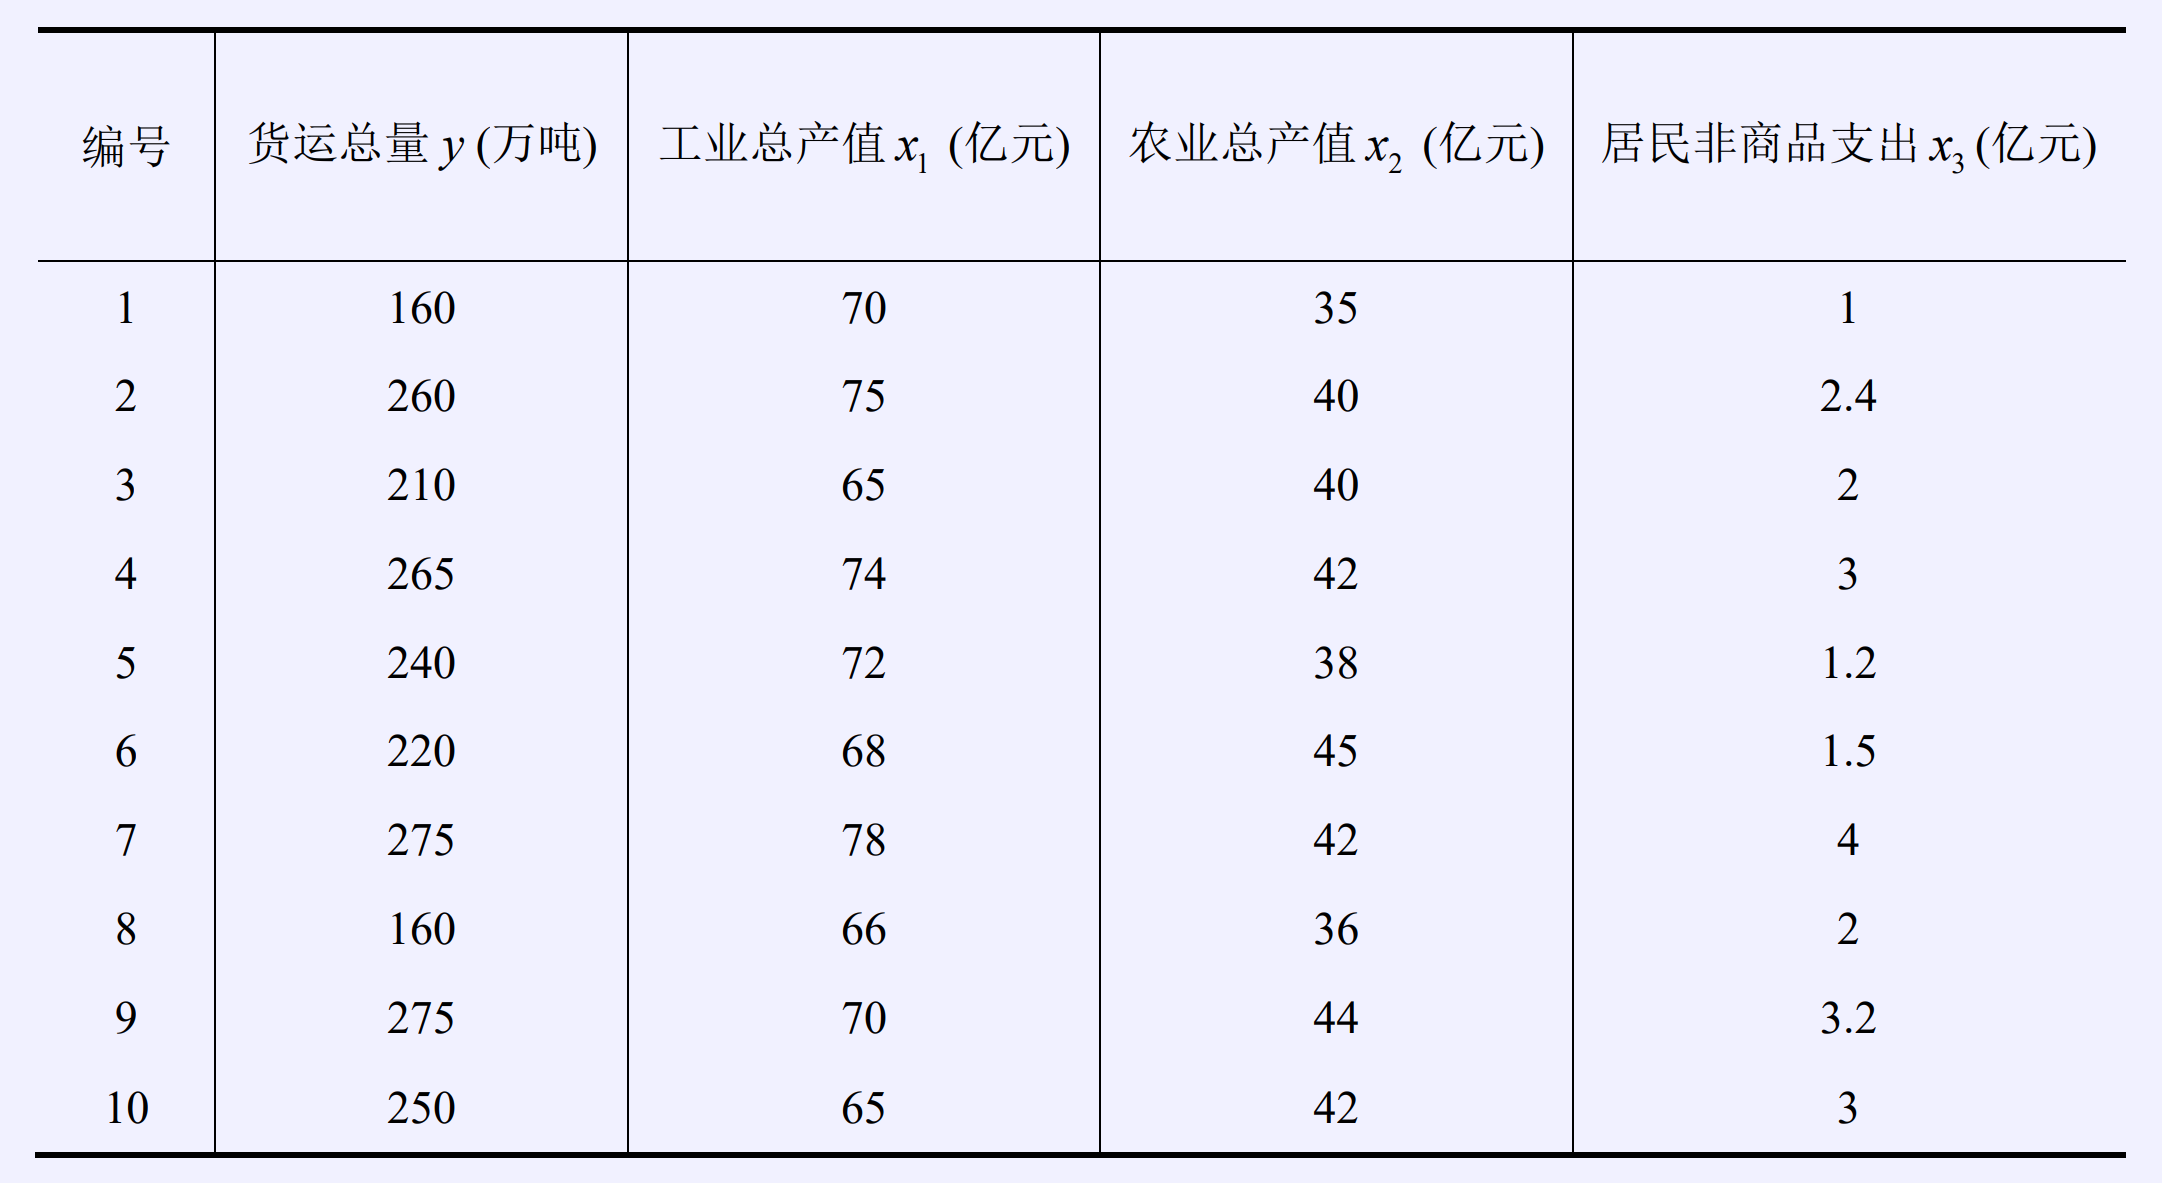
\includegraphics[height=7.6cm]{plot.png}	
\end{problem}

\begin{solution}
	先利用\textbf{R}建立数据集, 输入以下代码:
	\lstinputlisting[language=R]{code 1.r}
	\begin{enumerate}
		\item {\tt}    {\bf Solve.} 
		
		
		输入以下代码用于计算相关系数矩阵:
			\lstinputlisting[language=R]{code 2.r}
		得到输出结果如下,即$y,x_1,x_2,x_3$的相关系数矩阵:
        	\lstinputlisting[language=R]{result 1.r}
       
		\item {\tt }   {\bf Solve.}
		 
		 
		 继续输入以下代码:
			\lstinputlisting[language=R]{code 3.r}
		 输出后可以得到三元线性回归方程为:\[ y = 3.754x_1 +7.101x_2 + 12.447x_3-348.280. \]
		\item {\tt}    {\bf Solve.} 
	
	
	继续输入以下代码:
		\lstinputlisting[language=R]{code 4.r}
		得到输出如下:
			\lstinputlisting[language=R]{result 2.r}
           Multiple R-squared和Adjusted R-squared这两个值我们常称之为“拟合优度”和“修正的拟合优度”,指的是回归方程对样本的拟合程度。在这里我们可以看到修正的拟合优度为0.7083,比较接近1,说明拟合程度较好。
		\item {\tt }   {\bf Solve.}
		  
		  
		  由第3问的输出结果的最后一行可以看到, \textbf{F}检验的p值为$0.01487 < 0.05$,故在显著性水平0.05下, 我们认为通过回归方程整体的显著性检验。
		\item {\tt}    {\bf Solve.} 
		 
		 
		 由第3问的输出结果可以看出, $x_1,x_2$的p值分别为0.1002和0.0488,说明回归系数较显著。而$x_3$的p值为$0.2835>0.05$, 说明$x_3$的回归系数不显著,应该予以剔除。
		
		\item {\tt }   {\bf Solve.}
		
		重新输入以下代码:
		\lstinputlisting[language=R]{code 5.r}
		运行后可以得到
		\lstinputlisting[language=R]{result 3.r}
		故重新建立的回归方程为:
     	\[ y = 4.676x_1 +8.971x_2 - 459.624. \]
     	由输出结果的最后一行可以看到, \textbf{F}检验的p值为$0.006718 < 0.05$,故在显著性水平0.05下, 我们认为通过回归方程整体的显著性检验。由系数表可知, 各个回归系数的p值较小, 说明回归系数的显著性较高。
		\item {\tt}    {\bf Solve.} 
		\lstinputlisting[language=R]{code 6.r}
		提交后输出得到:
		\lstinputlisting[language=R]{result 4.r}
		因此, $x_1$的置信度为$95\%$的置信区间为$\left(1.234941,8.11632\right)$, $x_2$的置信度为$95\%$的置信区间为$\left(4.294268,13.64765\right)$.
		
		\item {\tt }   {\bf Solve.}
		
		
		重新输入以下代码, 对样本进行标准化之后求回归方程:
		\lstinputlisting[language=R]{code 7.r}
		输出后可以得到标准化后的回归方程为:
			\[ y = 0.4792x_1 + 0.6765x_2 - 7.552\times{10}^{-16}. \]
		
		
		\item {\tt}    {\bf Solve.} 
		
		重新输入以下代码:
		\lstinputlisting[language=R]{code 8.r}
		输出后可以得到:
		\lstinputlisting[language=R]{result 5.r}
		即令$x_{01}=75,x_{02}=42,x_{03}=3.1$时, 得到$\hat{y_0} = 267.829$. 同时置信区间为$ \left(204.4355,331.2225\right) .$
		
		\item {\tt }   {\bf Solve.}
		
		根据前面的分析,虽然$R^2$的值较大,但并不能说明回归方程显著,我们还需要通过对回归方程以及其系数进行检验。当一个回归方程通过显著性检验之后,也并不能说明这个方程中所以自变量都对因变量$y$有显著影响,还需对回归系数进行检验。
	\end{enumerate} 
\end{solution}

\end{document}
